As described above, we plan a suite of comprehensive simulations of a
large variety of stellar explosions: core-collapse and Type Ia
supernovae, XRBs, and the curious black widow pulsars.  Our simulation
codes are well-matched to these studies.  


XRBs and SNe Ia (both the sub-Ch and WDWD models) using our
codes \maestro\ and \castro.  All the problems we
describe are inherently three-dimensional, requiring large resources.
Our codes are running on titan today, and they perform and scale
well.  The starting point for all the simulations proposed are in
place.  We are ready to run.

The calculations we describe in further detail here are INCITE--class \MarginPar{needs updating}
for two reasons.  First, as is often the case in astrophysics, we can
never capture all the length-scales that come into play in these
stellar explosions, for example, the turbulent dissipation scale in
the convective regions is often quite below our grid resolution.  As a
result, we need to push to higher-and-higher resolution to assess
whether our results are converged.  This high resolution demands a lot
of computational resources---the type that only INCITE can provide.
Second, the temporal scales we need to model are equally impressive.
For the XRB simulations, we would like to model a second of evolution.
At our current resolution (6~cm), we would need over a million
timesteps (and that is with the large efficiency gain we get through
the low Mach model).  Since there is no parallel-in-time equivalent to
domain decomposition, we need to run a big problem for long amounts of
time on the machine---again, a feat only possible through INCITE.
Finally, we want to push the realism of the physics, in particular,
our reaction networks.  This will only be feasible by offloading some
of the reaction expense to the GPUs.

A key part of our collaboration is the emphasis on using GPUs
to accelerate the microphysics.  Both the Stony Brook and ORNL
groups have been working on this independently, and through this
proposal, we will unite our efforts to produce a set of community
GPU accelerated microphysics.  We will explore OpenACC, OpenMP 2.5,
and CUDA libraries to accomplish these goals, with an eye toward
summit.


The basic motivation for our science problems was given in the
previous section.  Here we begin by discussing the milestones we hope
to achieve in each year and then we give specific details about the
number and size of the simulations we plan to run.  We note that because
we have preliminary calculations of each of the problems we propose to
run, we can base our time requests on existing simulations from titan
(here Mh = mega-hours).  Also, there is a pattern to our milestones:
one milestone for each of the major topics per year (XRBs, sub-Ch,
WDWD, ...) with GPUs toward the end of the year, and the addition of 
new physics in years 2 and 3.  \MarginPar{read this}

\begin{tightitem}
\item {\bf Year 1: 115 Mh total }
%
\begin{tightitem}
\item \castro\ WD merger and collision simulations using realistic networks (10 Mh)
\item \maestro\ XRB convection calculations using large domains and realistic initial models (15 Mh)
\item \castro\ XRB flame calculations studies, including the first-ever 3D calculation (10 Mh)
\item \maestro\ sub-Chandra convection calculations (10 Mh)
\item \flash\ sub-Chandra explosion calculations (10 Mh)
\item \castro\ The first 3D radiation-hydro BWP calculations (5 Mh)
\item \maestro\ Urca calculations (5 Mh)
\item \chimera\ ccSNe calculations (50 Mh)
\end{tightitem}
%
\item {\bf Year 2: 130~Mh total}
%
\begin{tightitem}
\item WD merger simulations (10 Mh)
\item XRB convection calculations (15 Mh)
\item XRB flame calculations (15 Mh)
\item sub-Chandra convection calculations (10 Mh)
\item sub-Chandra explosion calculations (10 Mh)
\item BWP calculations (10 Mh)
\item Urca calculations (10 Mh)
\item ccSNe calculations (50 Mh)
\end{tightitem}
%
\item {\bf Year 3: 150~Mh total}
%
\begin{tightitem}
\item WD merger simulations (10 Mh)
\item XRB convection calculations (10 Mh)
\item XRB flame calculations (25 Mh)
\item sub-Chandra convection calculations (10 Mh)
\item sub-Chandra explosion calculations (10 Mh)
\item BWP calculations (15 Mh)
\item Urca calculations (10 Mh)
\item ccSNe calculations (60 Mh)
\end{tightitem}
%
\end{tightitem}

\begin{figure}[t]
\centering
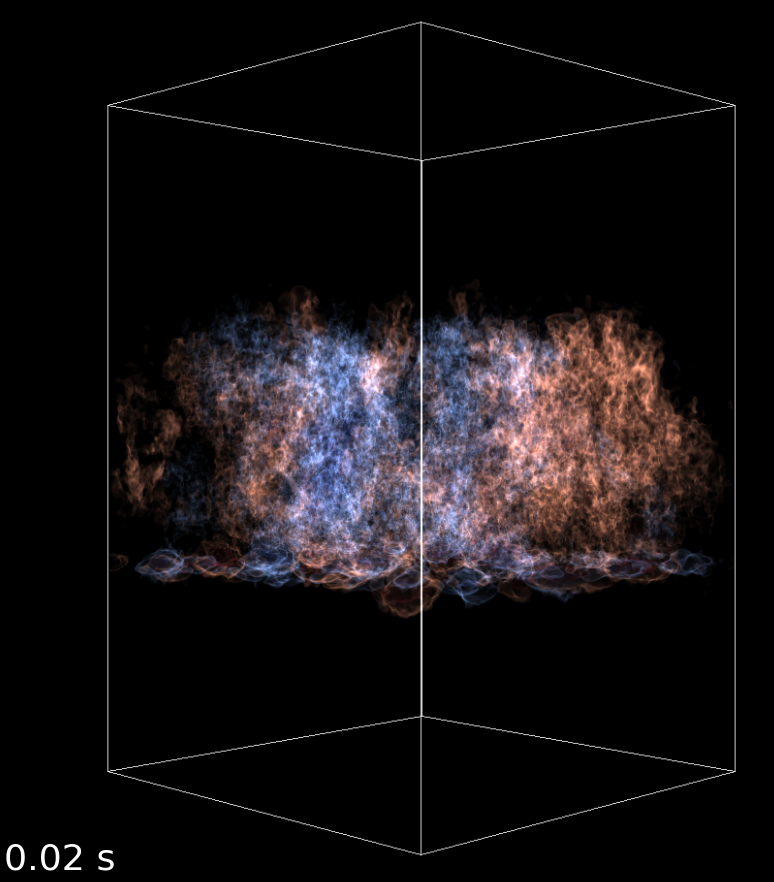
\includegraphics[width=0.28\linewidth]{xrb_compact}
\hspace{0.2em}
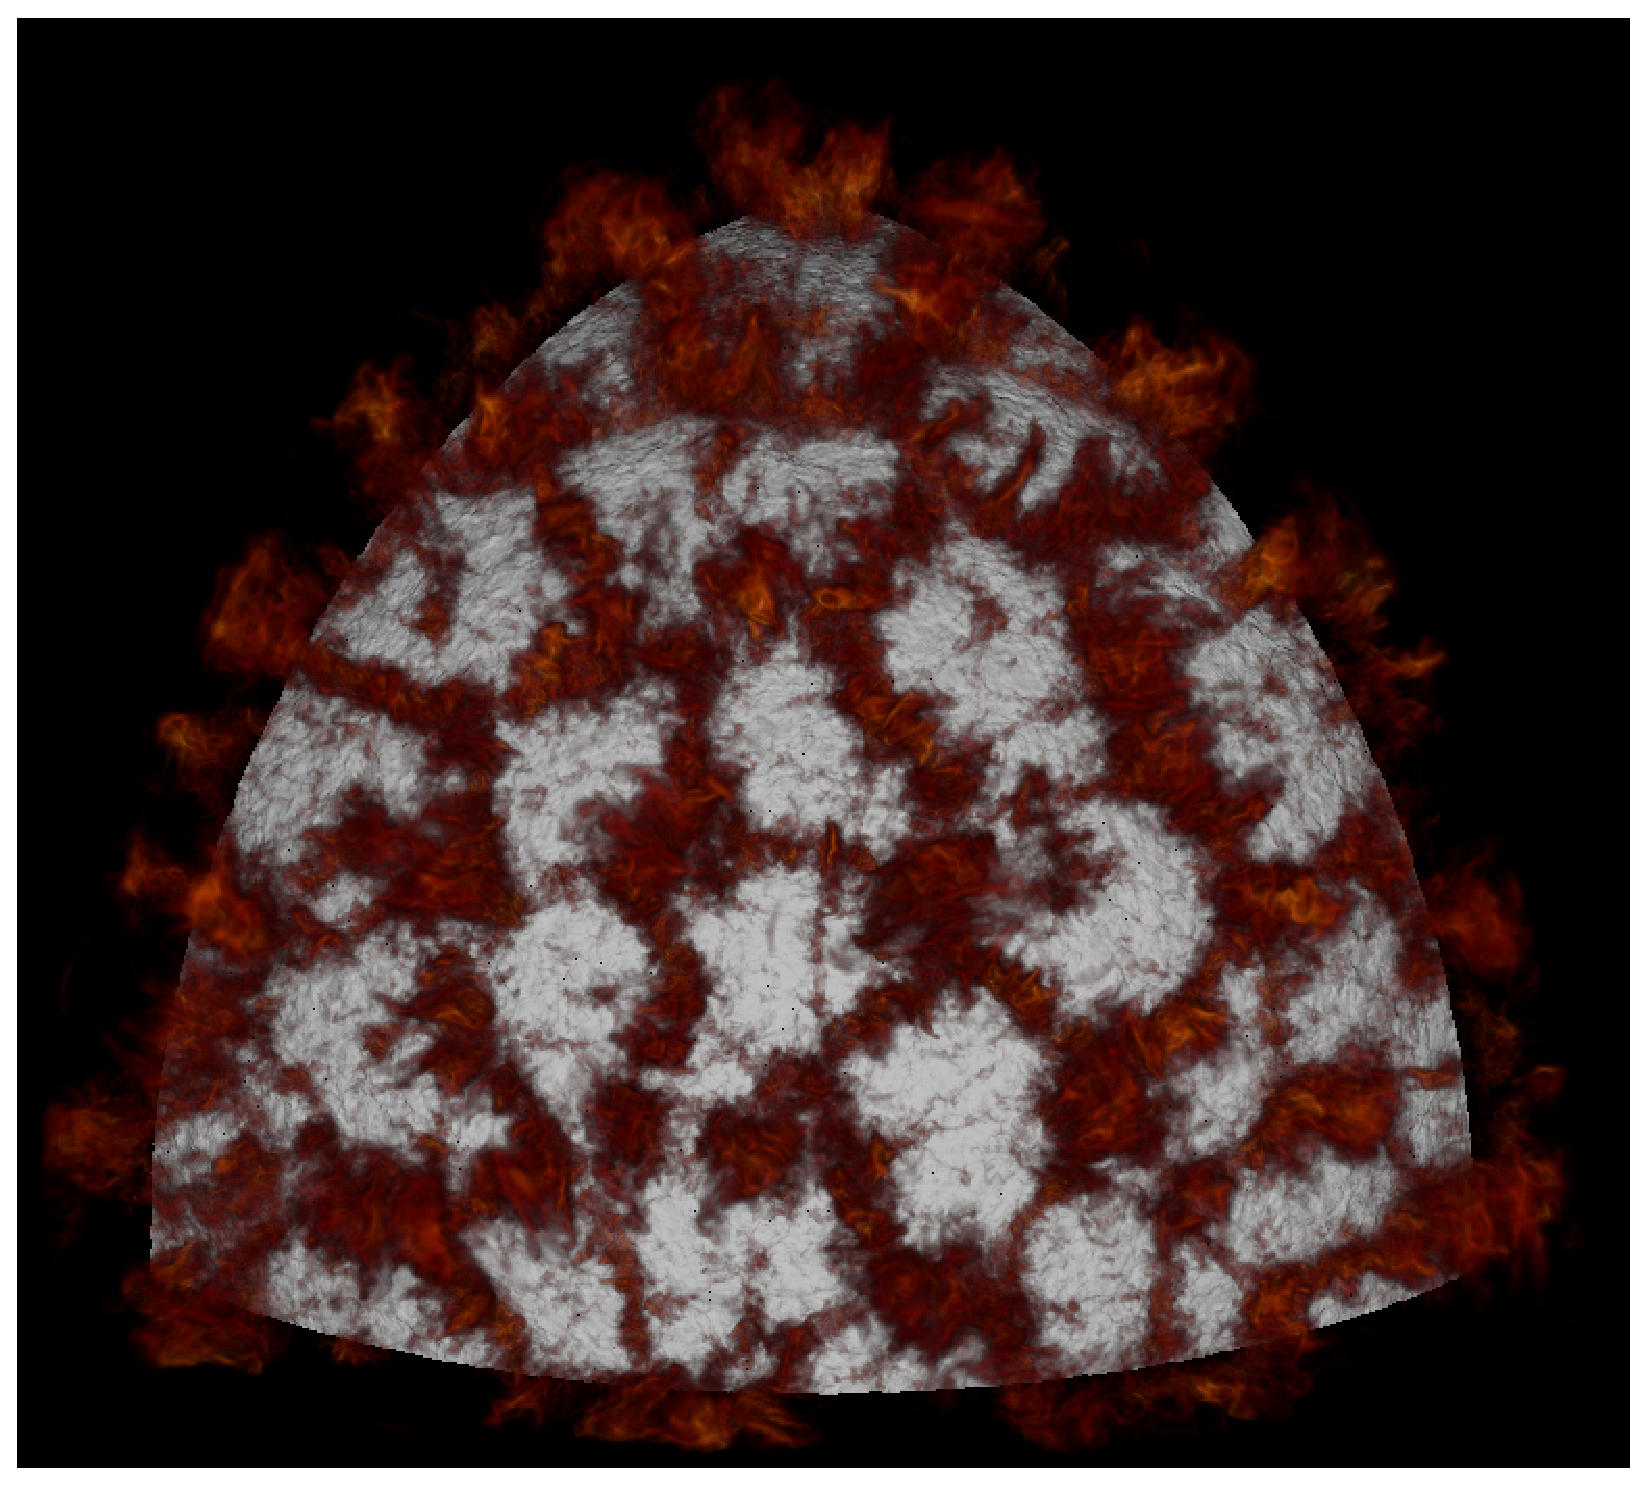
\includegraphics[width=0.28\linewidth]{ConvPlumes}
\hspace{0.2em}
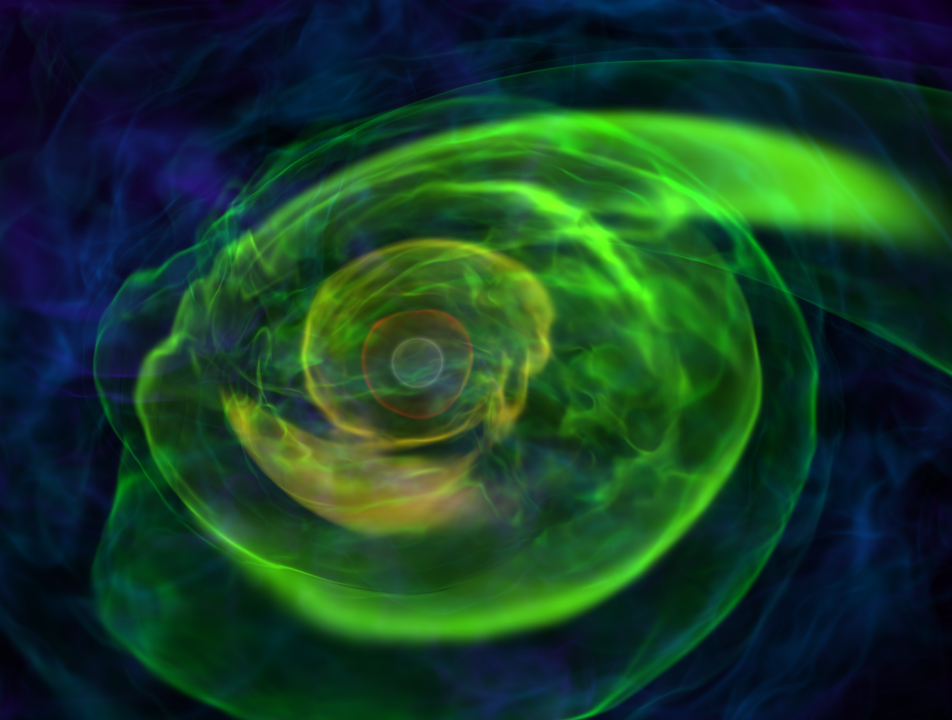
\includegraphics[width=0.4\linewidth]{wdmerger_08030_new.png}
\caption{\label{fig:current-runs} (top left) Vertical velocity showing the
  convective structure in a \maestro\ XRB calculation.  (top right)
  Convective plumes in a \maestro\ sub-Ch calculation.  (left)
  Snapshot of a \castro\ simulation of the merger of two white dwarfs,
  with 0.90 and 0.81 solar masses. The contours represent density
  levels. The star on the upper left is disrupting and accreting onto
  the other star.}
\end{figure}


\paragraph{SNe Ia simulations: }  

Our simulations of merging WDs will continue.  Our current work has
focused on just a few mass ratios and pure C/O WDs.  There are a lot
of unknowns in the WDWD system, and we will use the INCITE time to
explore the parameter space.  In the proposed period, we will greatly
expand the range of masses considered and we will also switch to more
realistic initial models with a layer of He on the surface.  The He is
more explosive, so this could trigger prompt explosions, as observed
by some other groups.  With our high resolution, enabled by the AMR in
\castro, we can understand with unprecidented detail whether the
conditions for detonation are achieved.  \MarginPar{Max self-consistent
  initial conditions?}

Finally, some simulations will be done of colliding white
dwarfs---these have been explored in the literature, but we can use
higher resolution and larger networks.  These are not as expensive as
the merger simulations, and will take only a small amount of the
requested time.


\paragraph{XRB simulations: } Resolving the burning in our XRB simulations requires
a resolution of 6 cm resolution.  Our current
\maestro\ calculation~\cite{xrb-3d} used a 512$\times$512$\times$768
grid, and required about 7.5 Mh on Titan.  As we showed in the paper
describing these results, simulation, this is wide enough to get a
good realization of the turbulent cascade in the convective region.
Our next set of models will use a more realistic initial model, from
the 1D studies of~\cite{woosley:2004}.  Our original calculations used
a relatively high base density for the H/He layer ($2\times
10^6~\gcc$).  This new model is better motivated physically, and also
affords us the ability to compare to the 1D stellar evolution models
to understand how the accurate 3D treatment of convection alters the
dynamics.  We will also explore a large domain size---currently we
model 31~m laterally on the neutron star surface---we'd like to
explore a size closer to 50~m to see the development of more
convective cells.  These will give a clear picture of the dynamics of
the convection and allow us to answer the questions posed in the
previous section: how does the convection alter the nucleosynthesis?
and are ashes brought up to the surface where they can change the
observables?

Secondly, we want to explore larger networks.  This will be enabled by
the GPU network, which should absorb the expense of a larger network.
At the moment, we use a 10-isotope network that captures the hot-CNO H
burning, 3-$\alpha$ He burning, and some links to heavier elements and
the rp-process.  We've discussed networks of the size 25--40 nuclei
with colleagues in the nuclear astrophysics community, and we believe
that we can find an appropriate approximate network in that size
range.  This will give us more realistic energetics, and allow us to
get a better picture of the nucleosynthesis in the event.  We expect that
the GPUs will mostly offset the cost of a larger network.

The next line of development is to explore the propagation of the
flame front through the H/He layer on the NS with \castro.  We are
currently running exploratory 2D calculations here, and should be set
to begin 3D calculations in year 1.  Rotation is essential here.
These calculations begin by perturbing a region of the atmosphere,
driving the burning that will eventually ignite a flame.  While
diffusion spreads the heat to the unburned fuel, the absense of a
laterial hydrostatic equilibrium in the partially-degenerate
atmosphere drives a flow from the perturbed region across the star.
Left unchecked, this will quench the burning.  It is the Coriolis
force that retards this flow, setting up a geostrophic balance.  This
scale, the Rossby length, is about 1~km in the star---on the edge of
what we are able to resolve.  In contrast to the work
of~\cite{cavecchi:2013}, we will model the vertical dynamics, with an
eye toward understanding how turbulence affects the burning.  To make
the simulations tractable, we will start with high rotation rates
(which make the Rossby length smaller).  Over the 3-year course of the
proposed work, we will work on expanding the domain, sub-grid models,
and connecting these calculations to the \maestro\ convection
simulations.


\paragraph{ccSNe simulations: }


\paragraph{BWP simulations: }  Our calculations of BWPs are just beginning.
Our setup models the stellar companion (a low mass main-sequence star)
and illuminates it with an intense radiation field coming through the
boundary.  At the moment, we are doing using a gray flux-limited
diffusion (FLD) solver of \castro, but over the course of this
proposal, we will switch to multigroup FLD, and explore adding
additional moments to the radiation field in \castro\ (in particular,
the M1 approximation).  


\paragraph{Post processing and observables: }
%
For the SNe Ia models that we bring to explosion, we will use the \MarginPar{Dan?}
\sedona\ radiation transfer code to produce synthetic observables
(lightcurves and spectra)---the \sedona\ author Dan Kasen is a Co-I on
this proposal.  This post processing was done with many of the explosion 
models in the current INCITE allocation and the pieces are in place for this
workflow. We do not expect \sedona\ to require a lot of compute
time for these models.


\paragraph{Exploratory simulations: }
%
We are
capable of modeling all phases of these explosive phenomena.  As a
result, when a new idea is promoted in the field, we will be in an
excellent position to explore it through detailed high-resolution
simulation.  We will keep pace with the field and propose some add-on
calculations in later year renewals.  One example already placed in
our milestones is the URCA calculation.



